\proposedbox{
\section{Important technical documents published by MSL}

MSL self-publishes various types of document, such as our Technical Guides and Callaghan Innovation Technical Reports. These publications need to remain accessible, which can be achieved by archiving publications as digital records in an appropriate scientific repository. 

The preferred repository for MSL publications is \href{https://zenodo.org}{Zenodo}.  

\subsection{Zenodo}
\label{ss:zenodo}
Zenodo is an open-science repository created and operated by \href{https://home.cern/}{CERN}. It is available for use by anyone. 

\subsubsection{MSL Communities} MSL keeps collections of archived publication records on Zenodo, which are called \href{https://help.zenodo.org/docs/communities/about-communities/}{communities}. There are MSL communities for (\textbf{URLs will be available}):
\begin{itemize}
    \item Technical Guides
    \item Technical Reports
\end{itemize}

MSL's communities are owned and curated by the Chief Metrologist (\textbf{to be confirmed}). 

Publication records are always deposited in Zenodo by an individual. 

After deposit, a record should be submitted to a community. The community's curator is responsible for accepting each submission. 

\subsubsection{Accounts} Individuals must have a personal account to use Zenodo. There are different ways to create an account (via existing ORCID or Github accounts, or by creating an account directly with Zenodo), see \href{https://help.zenodo.org/docs/get-started/create-an-account/}{here}.

\subsubsection{Publication records}
Individual publications (e.g., a particular technical report or technical guide) will each require an `upload' (Zenodo teminology). 

When a publication is uploaded for the first time, the record must be named and a DOI will be issued. A lot of metadata can be provided at this stage. Everything can be saved, and re-edited,  during this process until the submission is \textit{published} on Zenodo. 

After publication, changes cannot be made to the publication itself and the upload cannot be easily removed (deleted). Some changes to the metadata are permitted. 

However, revised versions of an earlier upload can be deposited. This is done by the individual who made the initial upload. After selecting the link to an upload, the option of depositing a revised version becomes available. The new version is issued with a distinct DOI.    

\subsection{The FAIR principles}
The FAIR principles can be applied to enhance the value of digital assets, like our publications, in terms of use by others \cite{FAIR}. 

In relation to MSL publications, they can be interpreted as follows:
\begin{description}
	\item[Findable: ] A document must have a unique identifier (e.g., for searching and indexing purposes).  A Digital Object Identifier (DOI) is appropriate \cite{doi}. Several public science repositories issue a DOI when a document is deposited. Using one of these also takes care of the `A' principle, because the repository will also ensure that the document remains accessible.
	
	Authors should also be identified: each author should include their ORCID in the document \cite{orcid}.
	
	\item[Accessible: ] A document must be accessible (online). A distinction is made between knowing that a document exists (e.g., finding it in a search) and accessing it. 
	
	A document may still be protected from unauthorised use (e.g., by encryption) so openness is not implied.
	
	\item[Interoperable: ] A variety of applications should be able to use of the document. Publishing documents in PDF format (or better, in the PDF-A format) ensures that prospective readers have a choice of reading tools.
	  
	\item[Reusable: ] We publish documents for others to read, but sometimes also to reuse or re-distribute. Without a clear statement about copyright and licensing, a reader does not know if we give permission for the material to be reused. Permission should be explicitly granted, with an indication of acceptable ways of doing so. The Creative Commons licence, described in \S\ref{s_copyright}, is suitable. 

The provenance of work needs to be acknowledged too. Advice on how to cite (reference) a work should be included. 

\end{description}  

\subsection{Guidelines}
\subsection{Technical reports}
The figure below shows the appearance of an MSL technical report. Note the hyperlink to the DOI, where copies of the report are available. The green icon after the author's name is the orcid icon and is a hyperlink to orcid.

\begin{center}
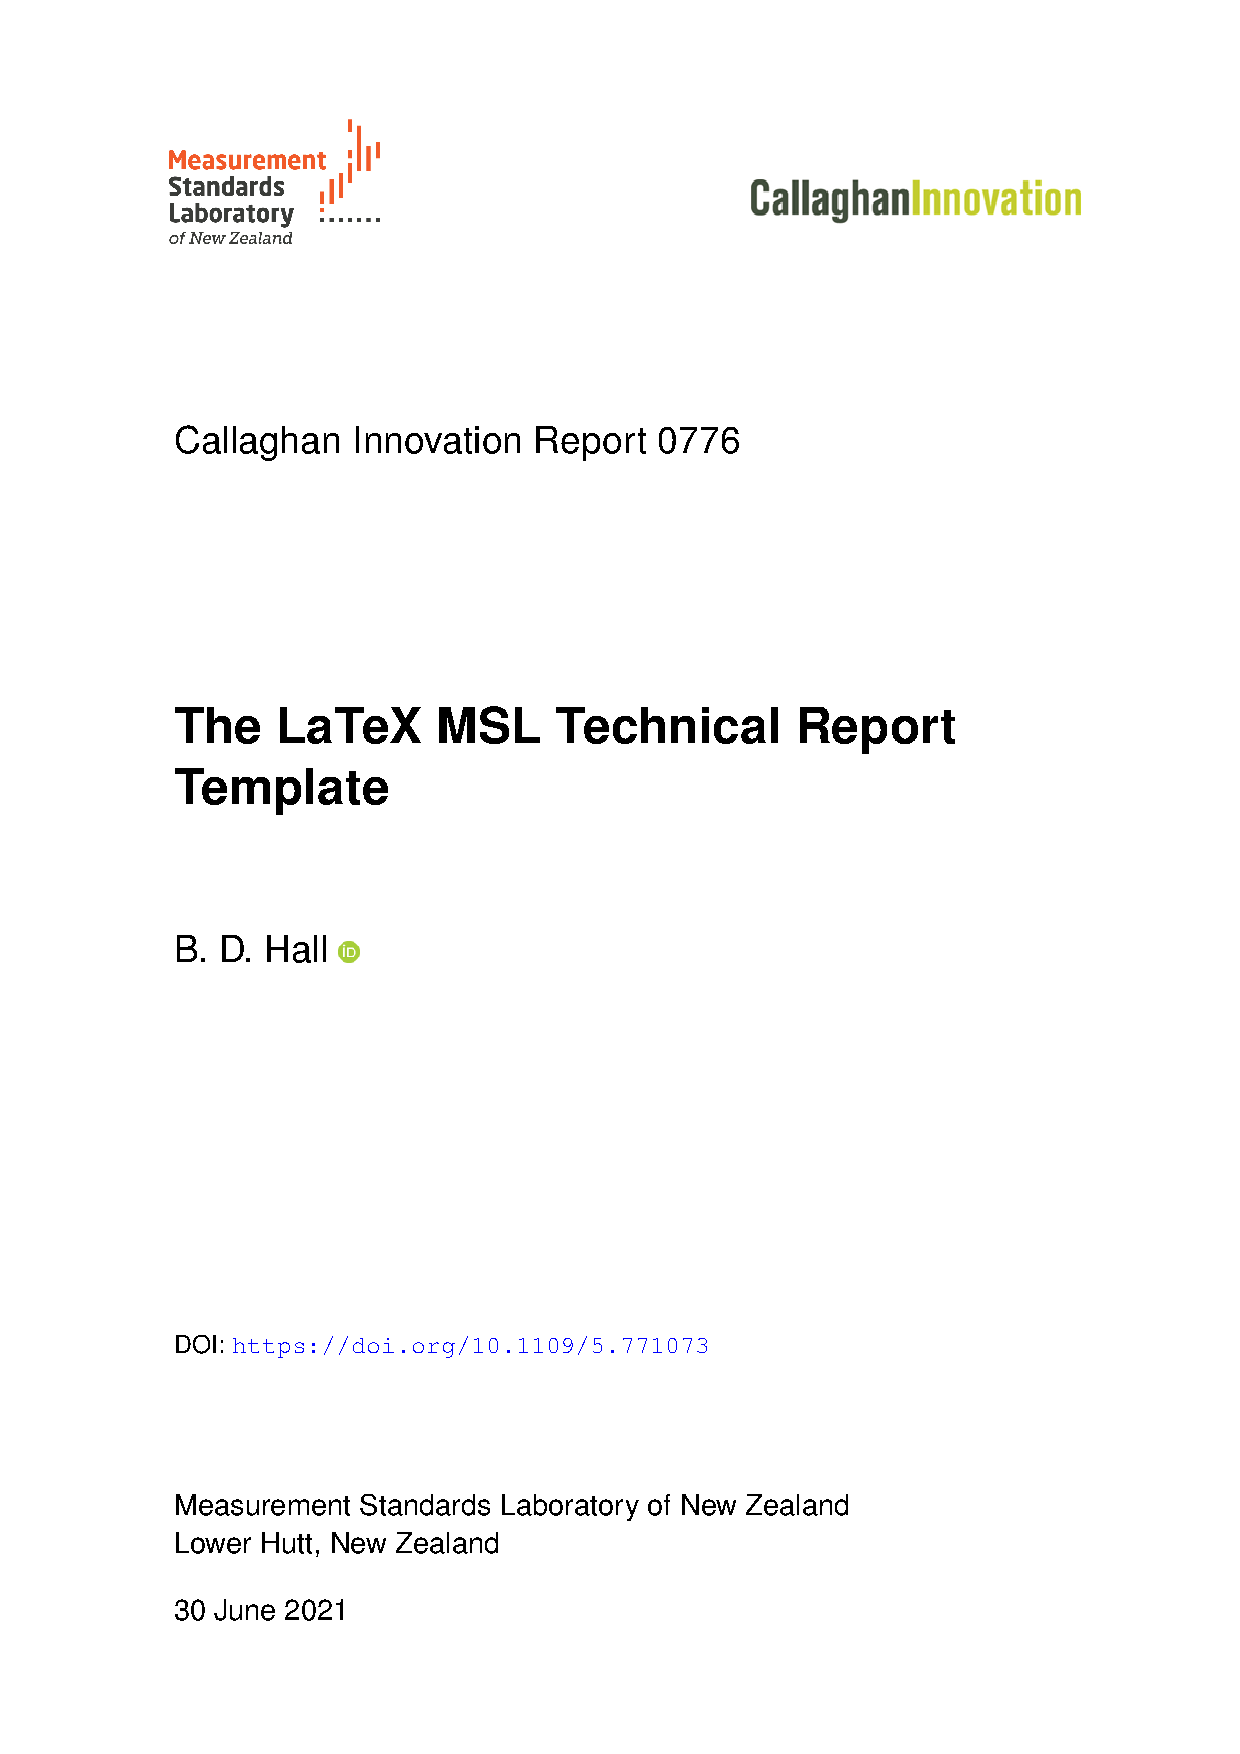
\includegraphics[scale=.5,page=1]{pictures/Report}
\end{center}

\newpage
The inside page of an MSL technical report repeats the title and includes a `reference', which suggests how the work can be cited, as shown below. The Creative-Commons licence is automatically placed after the summary / abstract material. 

\begin{center}
\includegraphics[scale=.5,page=2]{pictures/Report}
\end{center}

\subsection{Technical Guides}
The figure below shows the appearance of an MSL Technical Guide. The DOI is given in the header but not as a hyperlink.
\begin{center}
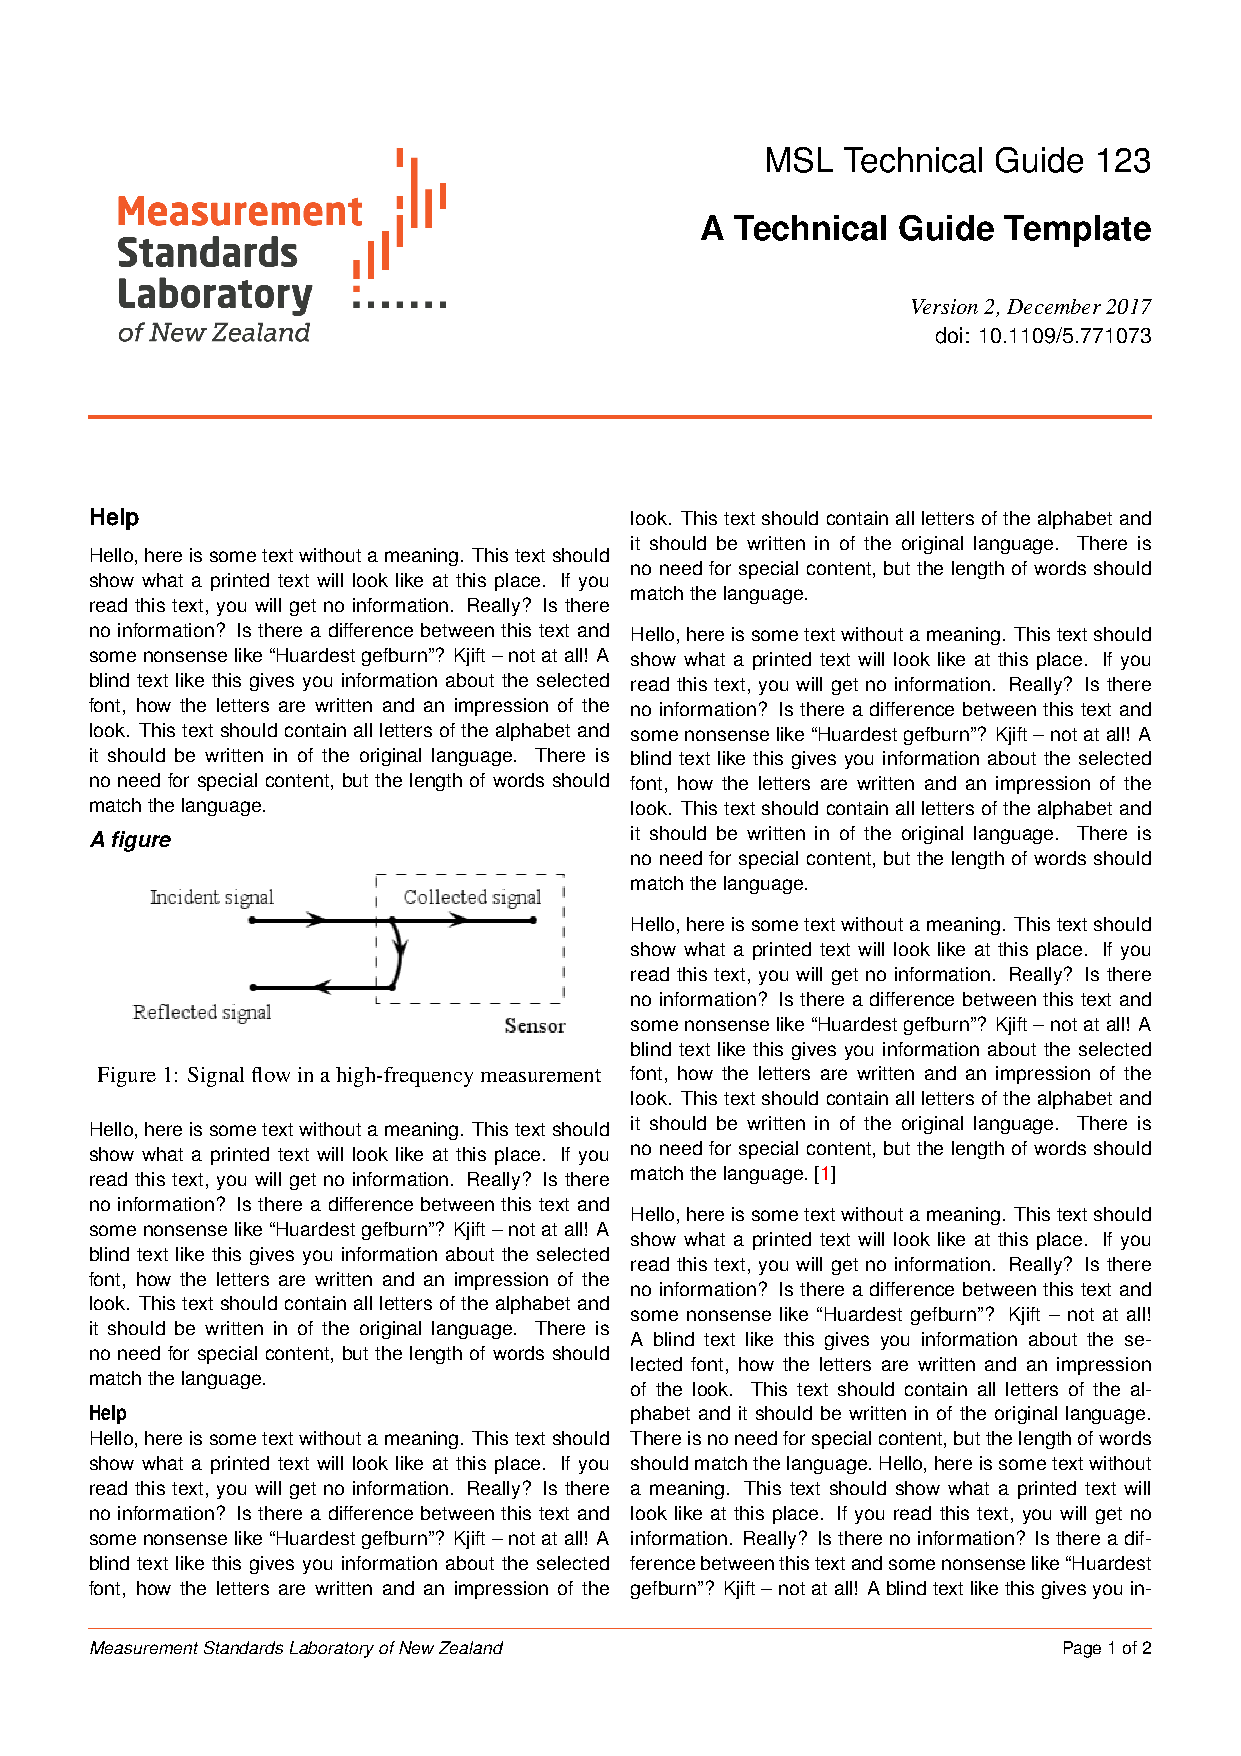
\includegraphics[scale=.5,page=1]{pictures/TG_Template}
\end{center}

\newpage
The last page of Technical Guide has an end-matter section where the names and orcids of the people who prepared the guide appear with other contact details. The doi is repeated here, but this time as a hyperlink. The Creative-Commons licence is automatically included.

\begin{center}
\includegraphics[scale=.5,page=2]{pictures/TG_Template}
\end{center}
}%